\subsection{dioganalsation}

The performance of the MPO construction can be compared with the exact diagonalisation of the hamiltonian for a given number of sites. To obtain a faithful results, the number of sites should be as high as possible. In practice, diagonalisation of large matrices becomes slow and memory consuming. The size grows exponentially in the number of sites: $d^{n} \times d^{n} $. A double takes 8 bytes of memory.A Rough estimated of the amount of RAM $R$ needed to store this complex array is:

\begin{equation}
    R = d^{2 n} \times 16 bytes
\end{equation}

Which means a 14 site chain already takes up  GB of RAM.

\todo{time complexity algoritms}




\subsubsection{norms}

\todo{trace norm, schatten p norm, ...}

The schatten 2 norm is used in the following analysis, dentoted by ${\| \cdot \|} _{2}$. In the figures the relative error $\epsilon$ is reported.


\def \expHBlock {\expH{4}{ $e^{- \beta \hat{H}_{n}}$   }{ {,,"...",} }{ {,,"...",} }{}{} }
\def \Mn {\mpo{4}{ {0,,,,0}  }{}{}{{0,0,1,0,0}}{}}


\begin{equation}
    \epsilon = \frac{  {  \left \|  \expHBlock - \Mn  \right \|} _{2}  }{ {  \left\|  \expHBlock \right \|}_2}
\end{equation}


\subsection{system size and cyclicity}

This norm can only be calculated for a finite number of sites. The influence of the number of sites for a linear  and cyclic \cref{benchmarking:systemsize} . As expected, the cyclic norm represents large systems better for the same number of sites. The linear norm keeps increasing with every added site.

Calculating the cyclic norm comes at the extra cost of contracting a cyclic tensor network. \todo{calculate complexity}

In this chapter, the cyclic norm will be given for M=8 sites.

\begin{figure}[H]
    \begin{subfigure}[]{\textwidth}
        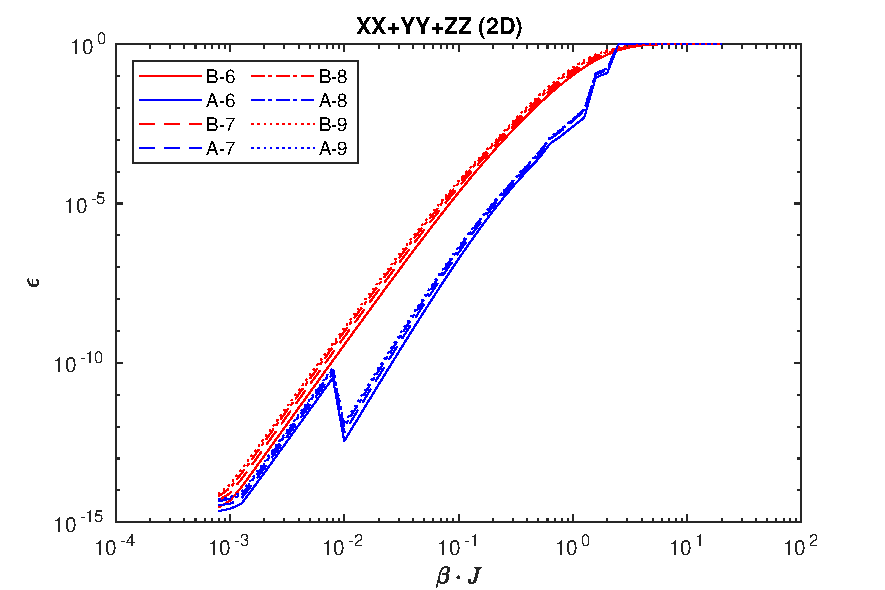
\includegraphics[width=\textwidth]{Figuren/benchmarking/keuze_norm/linear.pdf}
        \subcaption{test}
    \end{subfigure}

    \begin{subfigure}[]{\textwidth}
        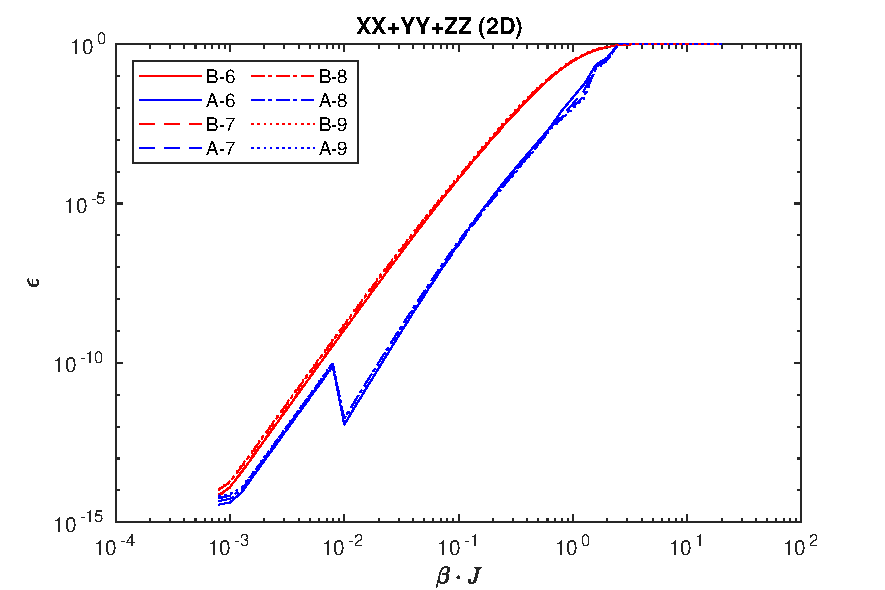
\includegraphics[width=\textwidth]{Figuren/benchmarking/keuze_norm/cyclic.pdf}
        \subcaption{test}
    \end{subfigure}
    \caption{test }
    \label{benchmarking:systemsize}
\end{figure}



\subsubsection{Ising}


\paragraph{optimal model parameters}



The first model used to benchmark the different types of MPO's is the transversal ising model. For type A the $\epsilon$ increases with
$\beta$. As expected, the relative error decreases with increasing order.

The behaviour of type B is more chaotic. The error increases no longer monotonously. For small values of $\beta$, the order is truncated.


\begin{figure}[H]
    \center
    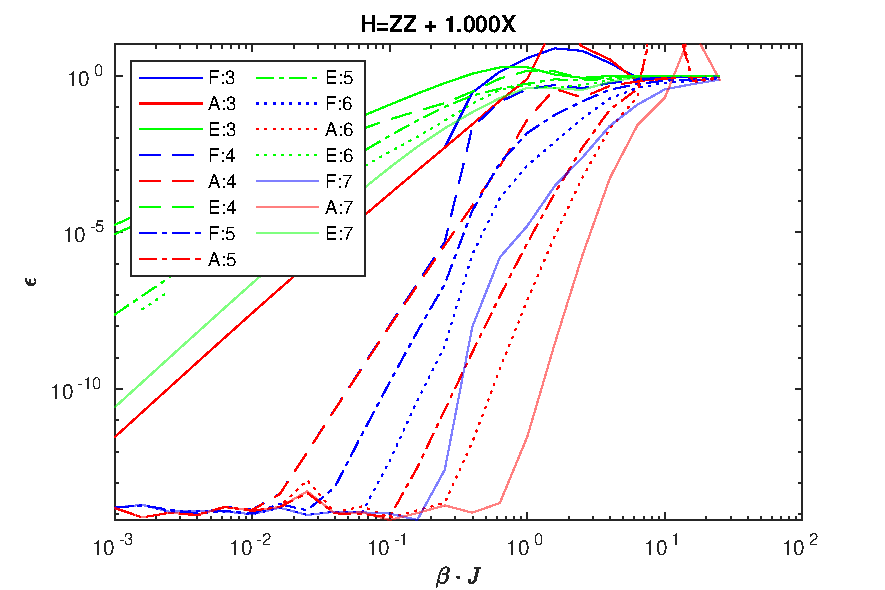
\includegraphics[width=\textwidth]{Figuren/benchmarking/t_ising.pdf}
    \caption{Comparison type A and B for Transversal Ising}
    \label{fig:benchmark:tising}
\end{figure}

\subsubsection{Heisenberg}

For the Heisenberg model, type A is also an improvement over type B. For large values of $\beta$, type A is not able to reproduce the exact


\begin{figure}[H]
    \center
    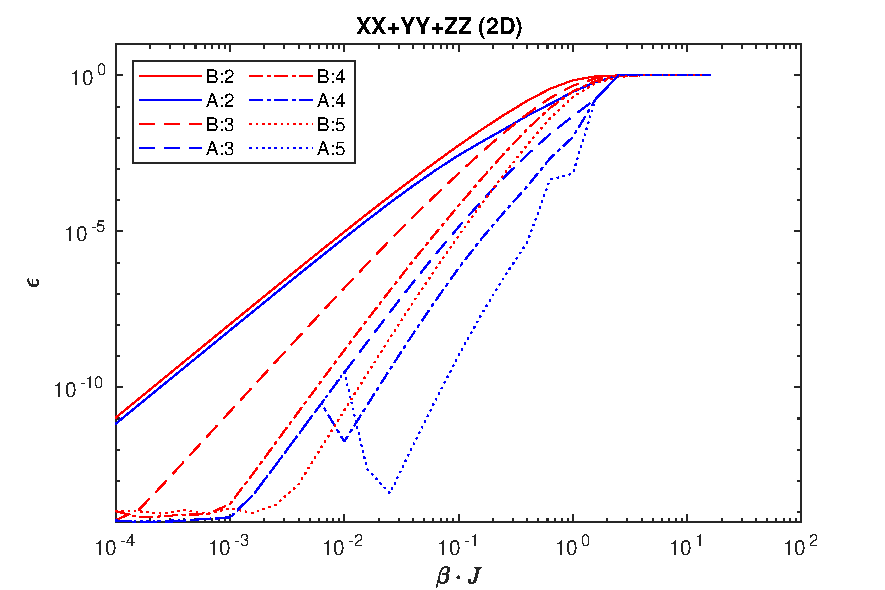
\includegraphics[width=\textwidth]{Figuren/benchmarking/heisXXX.pdf}
    \caption{Comparison type A and B for Heisenberg}
    \label{fig:benchmark:Heisenberg}
\end{figure}



\begin{figure}[H]
    \center
    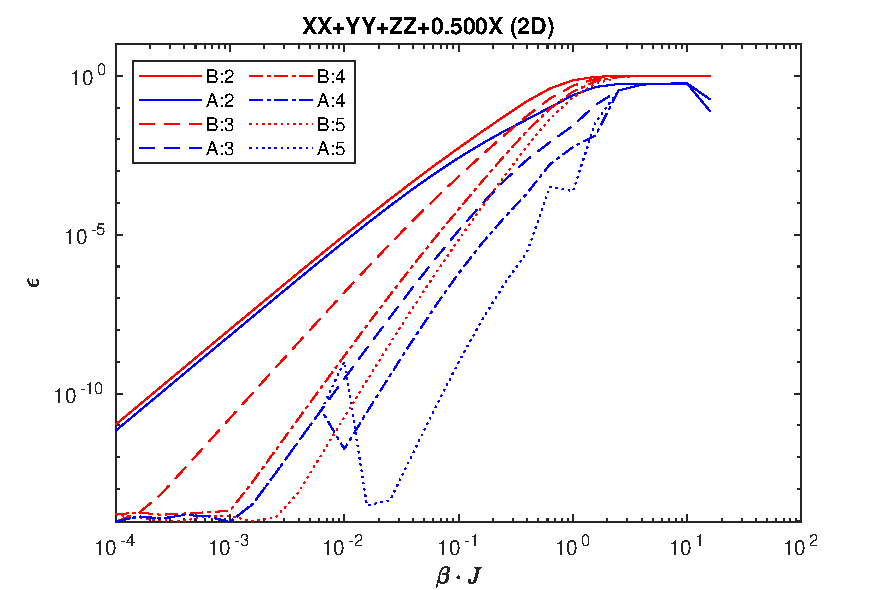
\includegraphics[width=\textwidth]{Figuren/benchmarking/t_heis_XXX.pdf}
    \caption{transversal XXX}
    \label{fig:benchmark:tHeisenberg}
\end{figure}


\todo{run with M=11}

\subsection{Random}

To give a representative overview for random hamiltonians, several simulations were run. The single site and nearest neighbourgh hamiltonians are generated by making hermitian matrices with random real and complex numbers between -1 and 1. In order to compare the different graphs, the engergy scale is set such that the norm of the 2 site hamiltonian is 1.


Clearly, the performance of type B is almost independent on the chosen random variables. For type A there is more variation. Still, A performs almost always better than B. As stated in the construction. no clear criterium is found for the truncation of odd orders (addition of double blocks). This can be seen for order 5  in some graphs.

For most of the trials, orders higher than 6 get truncated.

\begin{figure}[H]
    \begin{subfigure}[]{\textwidth}
        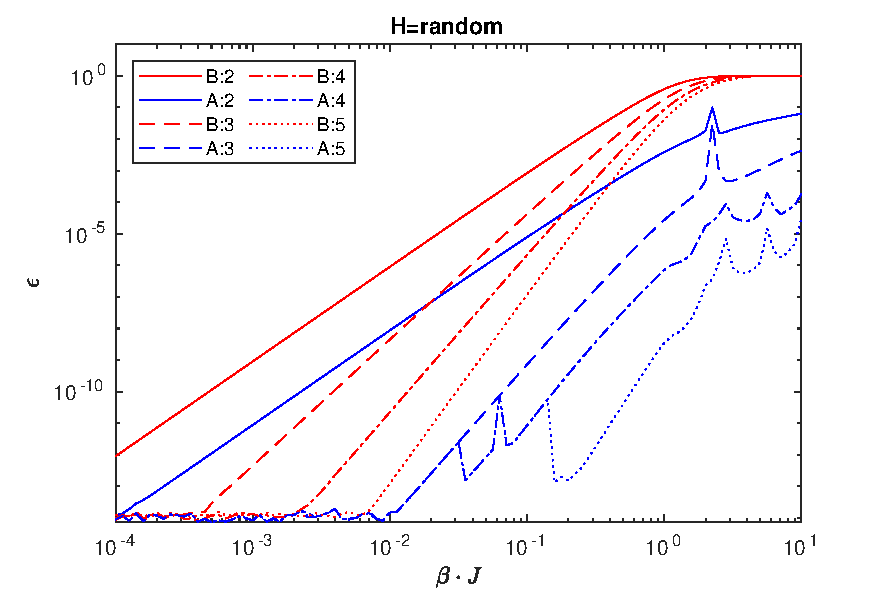
\includegraphics[width=\textwidth]{Figuren/benchmarking/rand_01.pdf}
        \subcaption{test}
    \end{subfigure}

    \medskip

    \begin{subfigure}[]{\textwidth}
        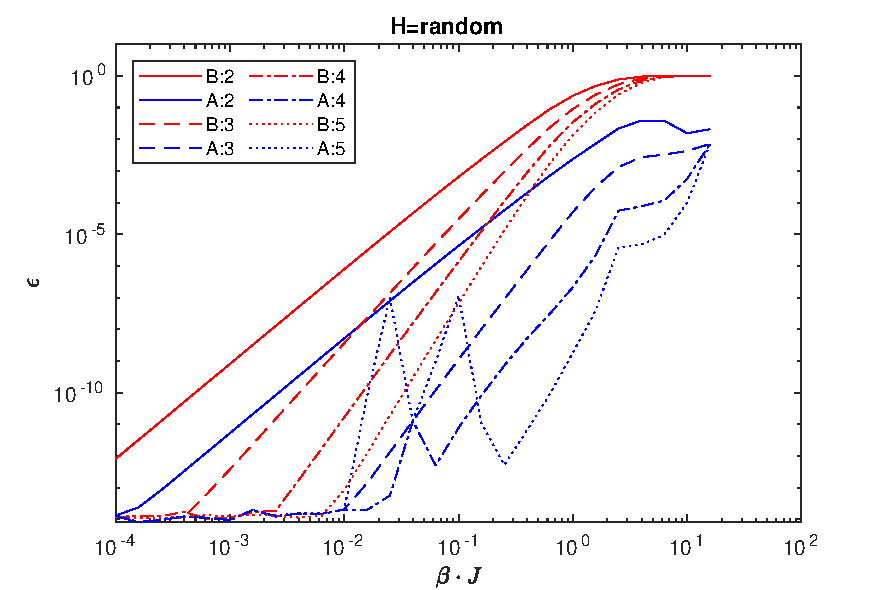
\includegraphics[width=\textwidth]{Figuren/benchmarking/rand_02.pdf}
        \subcaption{test}
    \end{subfigure}

    \caption{test }
\end{figure}

\begin{figure}[H]\ContinuedFloat
    \begin{subfigure}[]{\textwidth}
        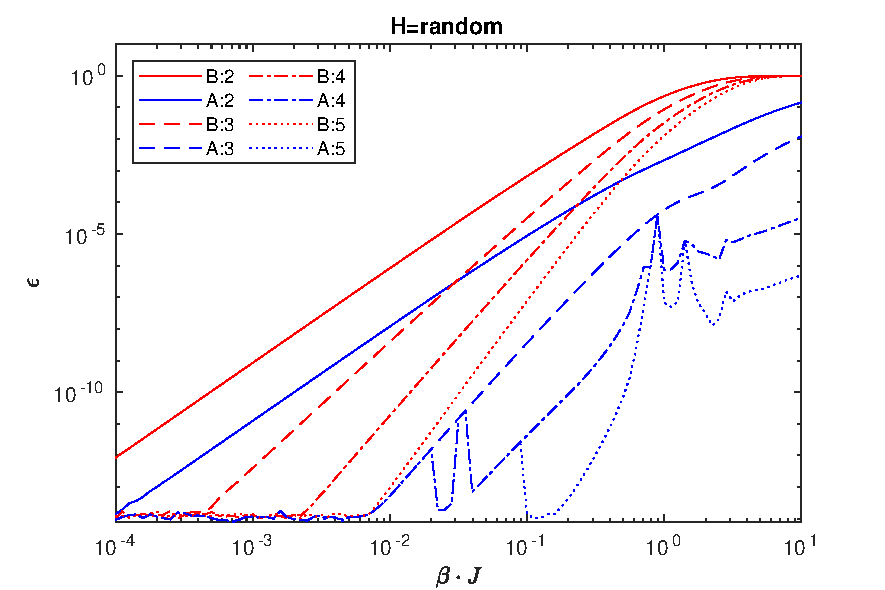
\includegraphics[width=\textwidth]{Figuren/benchmarking/rand_03.pdf}
        \subcaption{test}
    \end{subfigure}

    \begin{subfigure}[]{\textwidth}
        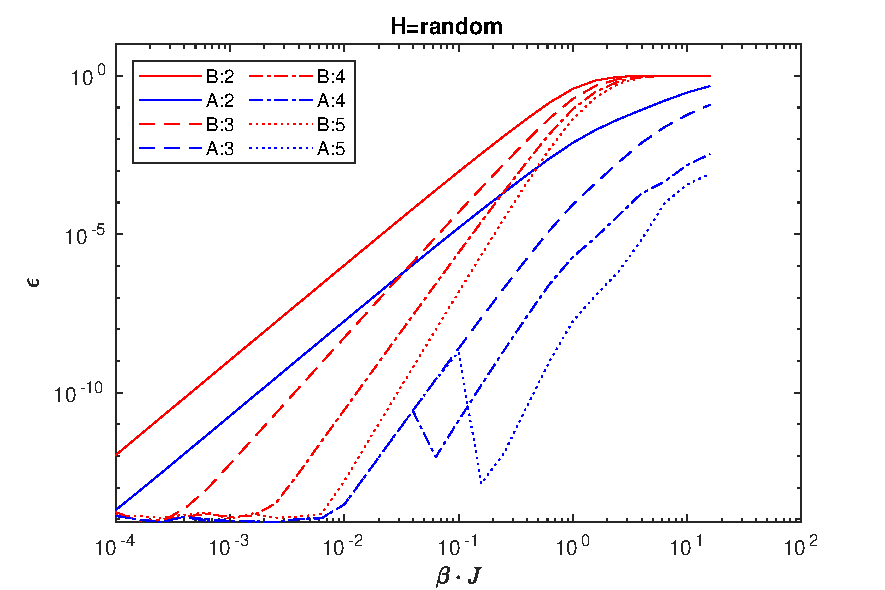
\includegraphics[width=\textwidth]{Figuren/benchmarking/rand_04.pdf}
        \subcaption{test}
    \end{subfigure}
    \caption{test (cont.) }
    \label{fig:benchmark:Random}
\end{figure}





\subsection{analytical results}